\documentclass{beamer}
\usepackage[utf8]{inputenc}
\usepackage{amsmath, amssymb}
\usepackage{graphicx}
\usepackage{mhchem}

\usetheme{Madrid} % You can choose other themes

\title{Previsão de Equilíbrios Químicos a Partir de Estruturas Atômicas}
\subtitle{Baseado em "Chemical Equilibria Can Be Predicted from Atomic Structures"}
\author{Ney Lemke}
\date{\today}

\begin{document}

\frame{\titlepage}

\begin{frame}{Previsão de Equilíbrios Químicos}
        Um dos principais objetivos da química é prever os equilíbrios das reações químicas.
        
        Isso envolve determinar as quantidades relativas de reagentes e produtos a partir de suas propriedades estruturais como:
        \begin{itemize}
            \item Massas atômicas
            \item Comprimentos de ligação
            \item Momentos de inércia
        \end{itemize}
        
        Neste contexto, focaremos em reações em fase gasosa, que são mais simples que reações em fase líquida.
\end{frame}

\begin{frame}{Equilíbrio Simples de Dois Estados}
        Considere o equilíbrio mais simples entre dois estados, A e B:
        $$ \ce{A <=>[\text{K}] B} $$
        
        Exemplos incluem: isomerização química, enovelamento de biopolímeros, ligação de um ligante. 
        A constante de equilíbrio $K$ é a razão das concentrações de partículas em cada estado no equilíbrio.
        A seta indica a direção, tornando $K = [B]/[A]$ inequívoco.
\end{frame}

\begin{frame}{Energia Livre de Gibbs e Potencial Químico}
        Para equilíbrios a temperatura (T) e pressão (p) fixas, a função apropriada é a energia livre de Gibbs:
        $$ dG = -SdT + Vdp + \mu_A dN_A + \mu_B dN_B $$
        
\end{frame}
        
\begin{frame}{Energia Livre de Gibbs e Potencial Químico}
        Em T e p constantes, a condição para equilíbrio é $dG = \mu_A dN_A + \mu_B dN_B = 0$. 
        Com $N_A + N_B = N_{total} = \text{constante}$, temos $dN_A = -dN_B$. 
        Assim, $(\mu_A - \mu_B)dN_A = 0$, o que implica que no equilíbrio:
        $$ \mu_A = \mu_B $$
        
        O objetivo é obter $\mu_A$ e $\mu_B$ a partir de modelos microscópicos.
\end{frame}

\begin{frame}{Relacionando $\mu$ com Funções de Partição}
        O potencial químico $\mu_A$ para a espécie A é dado por:
        $$ \mu_A = -kT \ln\left(\frac{q'_A}{N_A}\right) $$
        
        onde $q'_A$ é a função de partição da espécie A: $q' = \sum_j e^{-\epsilon_j/kT}$. 
        Similarmente para B:
        $$ \mu_B = -kT \ln\left(\frac{q'_B}{N_B}\right) $$
        
\end{frame}

\begin{frame}{Constante de Equilíbrio a partir das Funções de Partição}
        Substituindo na condição de equilíbrio $\mu_A = \mu_B$:
        $$ -kT \ln\left(\frac{q'_A}{N_A}\right) = -kT \ln\left(\frac{q'_B}{N_B}\right) \Rightarrow \frac{q'_A}{N_A} = \frac{q'_B}{N_B} $$
        
        Definindo a constante de equilíbrio $K = N_B/N_A$:
        $$ K = \frac{N_B}{N_A} = \frac{q'_B}{q'_A} $$
        
\end{frame}


\begin{frame}{Constante de Equilíbrio a partir das Funções de Partição}
        Pode-se também usar uma função de partição reduzida $q = e^{\epsilon_0/kT}q'$, onde $\epsilon_0$ é a energia do estado fundamental:
        $$ K = \left(\frac{q_B}{q_A}\right) e^{-(\epsilon_{0B} - \epsilon_{0A})/kT} $$
        
        Esta equação se aplica a partículas isoladas (fase gasosa), pois não considera interações intermoleculares.
\end{frame}

\begin{frame}{Energia e Densidade de Estados}
        Dois fatores contribuem para as populações de equilíbrio de A e B:
        \begin{itemize}
            \item Energias baixas
            \item Altas densidades de estados
        \end{itemize}
        
\end{frame}

\begin{frame}{Energia e Densidade de Estados}
        No equilíbrio, as moléculas individuais de A e B serão distribuídas de acordo com a distribuição de Boltzmann. O número de moléculas em um dado estado é determinado apenas pela energia, não pela forma (A ou B).


\end{frame}
\begin{frame}{Energia e Densidade de Estados}
        \begin{figure}
        \centering
         Conceptual representation of Figure 13.1
        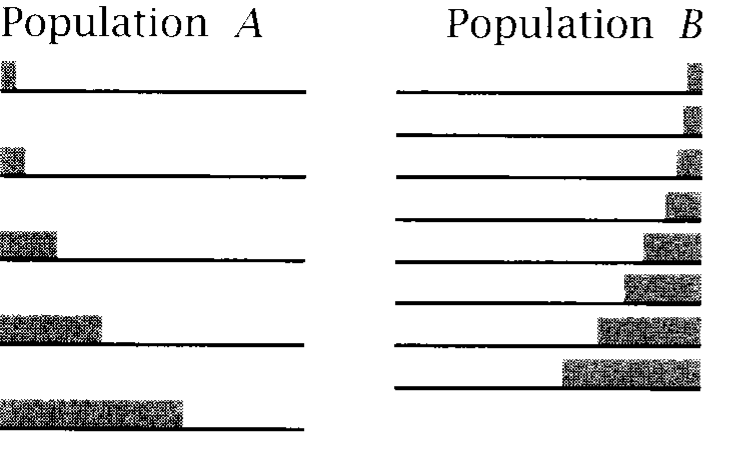
\includegraphics[width=0.6\textwidth]{figs/energylevels.png}
        \caption{Escadas de energia hipotéticas para o equilíbrio A $\leftrightarrow$ B. A pode ter o estado fundamental de menor energia, mas B pode ter maior densidade de estados.}
        \end{figure}
        Se os espaçamentos dos níveis de energia são menores para B do que para A, B pode ser a espécie com maior população total.
\end{frame}

\begin{frame}{Reação Geral: $aA + bB \rightarrow cC$}
        
        A condição para equilíbrio em T e p constantes é:
        $$ dG = \mu_A dN_A + \mu_B dN_B + \mu_C dN_C = 0 $$
         
        As restrições estequiométricas são:
        $ dN_A = -\frac{a}{c}dN_C $ e $ dN_B = -\frac{b}{c}dN_C $. 
        Substituindo, leva a:
        $$ c\mu_C = a\mu_A + b\mu_B $$
        
\end{frame}

\begin{frame}{Constante de Equilíbrio para Reação Complexa}
        Usando $\mu = -kT \ln(q'/N)$, obtemos:
        $$ \left(\frac{q'_C}{N_C}\right)^c = \left(\frac{q'_A}{N_A}\right)^a \left(\frac{q'_B}{N_B}\right)^b $$
         
        A constante de equilíbrio $K$ é:
        $$ K = \frac{N_C^c}{N_A^a N_B^b} = \frac{(q'_C)^c}{(q'_A)^a (q'_B)^b} $$
        
\end{frame}

\begin{frame}{Constante de Equilíbrio para Reação Complexa}
        Ou em termos de funções de partição reduzidas $q$ e energias de estado fundamental $\epsilon_0$:
        $$ K = \left(\frac{q_C^c}{q_A^a q_B^b}\right) e^{-(c\epsilon_{0C} - a\epsilon_{0A} - b\epsilon_{0B})/kT} $$
        
        Isso permite prever equilíbrios químicos a partir de estruturas atômicas.
\end{frame}

\begin{frame}{Diferença de Energia do Estado Fundamental $\Delta\epsilon_0$}
        Para calcular K, precisamos de $\Delta\epsilon_0 = c\epsilon_{0C} - a\epsilon_{0A} - b\epsilon_{0B}$.
        Um zero comum de energia é o estado totalmente dissociado. 
\end{frame}

\begin{frame}{Energia Vibracional e Energia de Ponto Zero}
        Energias vibracionais: $\epsilon_v = (v + 1/2)h\nu$. O nível de energia mais baixo acessível é $\epsilon_0 = (1/2)h\nu$ (energia de ponto zero). 
        Mudamos a referência para o ponto zero em vez do fundo do poço.
        A energia de dissociação $D$ é definida em relação ao fundo do poço ou ao ponto zero. O texto adota $D = -\epsilon_{0,\text{poço}} - (1/2)h\nu$, onde $\epsilon_{0,\text{poço}}$ é a energia no fundo do poço. 
        A função de partição vibracional (referência no ponto zero) é:
        $$ q_{vZ} = \frac{1}{1 - e^{-h\nu/kT}} $$
         
\end{frame}


\begin{frame}{Energia Vibracional e Energia de Ponto Zero}
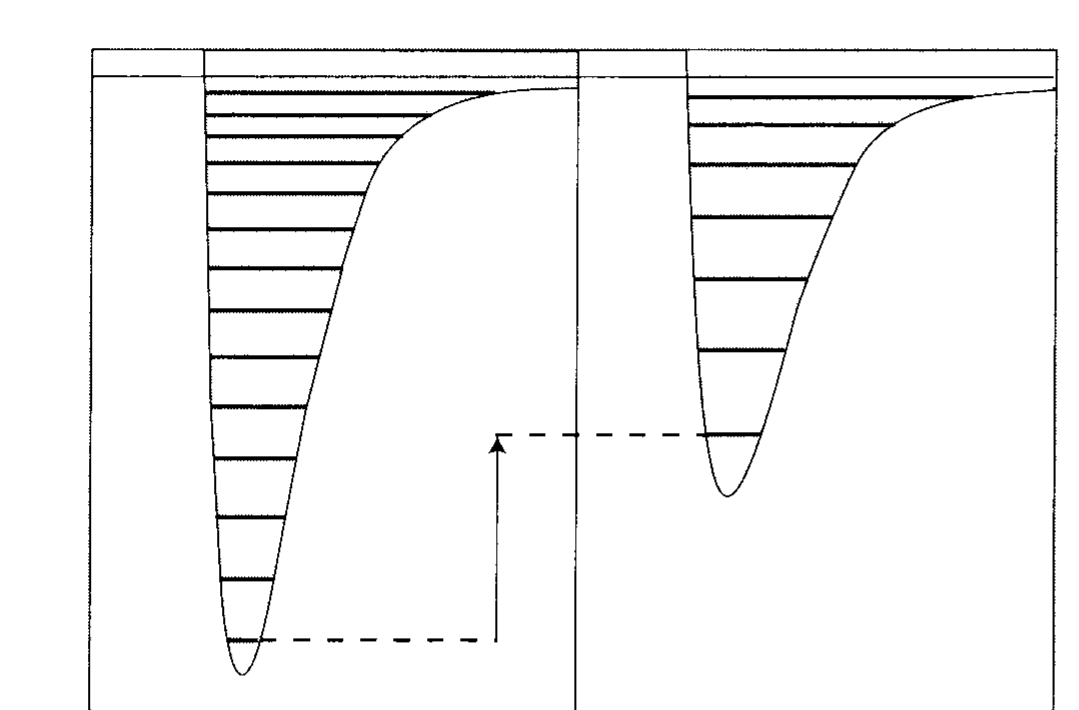
\includegraphics[width=0.6\textwidth]{figs/poco.png}
\end{frame}
    \begin{frame}{Energia Vibracional e Energia de Ponto Zero}
        O termo $q_{vibration} e^{-\epsilon_0/kT}$ (onde $\epsilon_0$ é a energia do fundo do poço) é substituído por $q_{vZ} e^{D/kT}$ (onde D é a energia de dissociação do estado de ponto zero ao dissociado).
        Assim, a constante de equilíbrio usa energias de dissociação $\Delta D_0$:
        $$ K = \left(\frac{q_C^c}{q_A^a q_B^b}\right) e^{\Delta D_0/kT} $$
        (onde $\Delta D_0$ é a diferença nas energias de dissociação (Produtos - Reagentes) medidas a partir dos seus respectivos estados de ponto zero).
\end{frame}

\begin{frame}{Exemplo: Reação de Troca $H_2 + D_2 \rightleftharpoons 2HD$}
    % This frame originally had no blocks, so it's kept as is.
    % Content from original frame:
    A constante de equilíbrio é:
    $$ K = \left(\frac{q_{HD}^2}{q_{H_2}q_{D_2}}\right) e^{\Delta D/RT} $$
    
    onde $\Delta D = 2D_{HD} - D_{H_2} - D_{D_2}$. 
    Energia de dissociação(D, a partir do ponto zero): $D_{H_2} = 431.8 \text{ kJ mol}^{-1}$, $D_{D_2} = 439.2 \text{ kJ mol}^{-1}$, $D_{HD} = 435.2 \text{ kJ mol}^{-1}$.
    $$ \Delta D = 2(435.2) - 431.8 - 439.2 = -0.6 \text{ kJ mol}^{-1} $$
    
\end{frame}

\begin{frame}{Exemplo: Reação de Troca $H_2 + D_2 \rightleftharpoons 2HD$}
    A $T=300K$, $e^{\Delta D/RT} = 0.79$. 

    $K = K_t K_r K_v e^{\Delta D/RT}$
    \begin{itemize}
        \item $K_t = \left(\frac{m_{HD}^2}{m_{H_2}m_{D_2}}\right)^{3/2} = \left(\frac{3^2}{2 \times 4}\right)^{3/2} = 1.19$
        \item $K_r = \left(\frac{\sigma_{H_2}\sigma_{D_2}}{\sigma_{HD}^2}\right) \left(\frac{I_{HD}^2}{I_{H_2}I_{D_2}}\right) = 4 \left(\frac{(6.13)^2}{(4.60)(9.19)}\right) = 3.56$ (com $\sigma_{H_2}=\sigma_{D_2}=2, \sigma_{HD}=1$)
        \item $K_v \approx 1$ (pois $h\nu/kT \gg 1$ para todas as espécies à temperatura ambiente)
    \end{itemize}
    
\end{frame}

\begin{frame}{Exemplo: Reação de Troca $H_2 + D_2 \rightleftharpoons 2HD$}
    $ K = (1.19)(3.56)(1)(0.79) = 3.35 $.
    À medida que $T \rightarrow \infty$, $K \rightarrow 4$. A mudança na simetria rotacional é o principal contribuinte.
\end{frame}

\begin{frame}{Potencial Químico e Pressões Parciais}
        $\mu = -kT \ln(q'/N)$. Fatorando $q' = q'_0 V$ e usando $V=NkT/p$:
        $$ \mu = -kT \ln\left(\frac{q'_0 kT}{p}\right) = kT \ln\left(\frac{p}{q'_0 kT}\right) $$
        
\end{frame}

\begin{frame}{Potencial Químico e Pressões Parciais}
        Isso pode ser escrito como:
        $$ \mu = \mu^{\circ} + kT \ln p $$
        
        onde $\mu^{\circ} = -kT \ln(q'_0 kT)$ é o potencial químico do estado padrão. $\mu^{\circ}$ depende da temperatura.
\end{frame}

\begin{frame}{Exemplo: Dissociação do Iodo $I_2 \rightleftharpoons 2I$}
    % This frame originally had no blocks, so it's kept as is.
    % Content from original frame:
    Calcular $K_p$ a $T=1000K$.
    Dados: $m_I = 2.109 \times 10^{-25} \text{ kg}$. Degenerescências eletrônicas do estado fundamental $q_{elec,I}=4, q_{elec,I_2}=1$. $\theta_{rot}=0.0537K, \theta_{vib}=308K, \Delta D = -35.6 \text{ kcal mol}^{-1}$ (para $I_2 \rightarrow 2I$, então $D_{I_2} = 35.6 \text{ kcal mol}^{-1}$).


\end{frame}

\begin{frame}{Exemplo: Dissociação do Iodo $I_2 \rightleftharpoons 2I$}
    $$ K_p = kT \frac{(q_{0I})^2}{q_{0I_2}} e^{-D_{I_2}/RT} $$
    (Note: a fórmula no livro é $e^{\Delta D/RT}$, com $\Delta D = D_{\text{produtos}} - D_{\text{reagentes}}$. Para $I_2 \rightarrow 2I$, $\Delta D = 2D_I - D_{I_2}$. Se $D_I$ é a energia para formar I atômico do zero de energia, e $D_{I_2}$ é a energia de dissociação de $I_2$, então $e^{-D_{I_2}/RT}$ é usado se $\Delta D$ no texto é $-D_{I_2}$.) O texto usa $\Delta D = -35.6 \text{ kcal mol}^{-1}$ diretamente na exponencial.

\end{frame}

\begin{frame}{Exemplo: Dissociação do Iodo $I_2 \rightleftharpoons 2I$}
    $e^{\Delta D/RT} = e^{-35600/(1.987)(1000)} = 1.66 \times 10^{-8}$. 
    Fatores das funções de partição ($q_0 = q_t q_r q_{vZ} q_e$):
    \begin{itemize}
        \item Rotacional ($I_2$): $q_{r,I_2} = T/(2\theta_{rot}) = 1000/(2 \times 0.0537) = 9310$.
        \item Vibracional ($I_2$): $q_{vZ,I_2} = (1-e^{-\theta_{vib}/T})^{-1} = (1-e^{-308/1000})^{-1} = 3.77$.
        \item Eletrônico: $q_{e,I}^2/q_{e,I_2} = 4^2/1 = 16$.
        \item Translacional: $\frac{q_{t,I}^2}{q_{t,I_2}} = \left(\frac{\pi m_I kT}{h^2}\right)^{3/2} = 3.01 \times 10^{33} m^{-3}$.
    \end{itemize}
    
\end{frame}

\begin{frame}{Exemplo: Dissociação do Iodo $I_2 \rightleftharpoons 2I$}
    $kT = 1.363 \times 10^{-25} m^3 atm$.
    $K_p = (1.363 \times 10^{-25})(1.66 \times 10^{-8}) \left(\frac{1}{9310}\right) \left(\frac{1}{3.77}\right) (16) (3.01 \times 10^{33}) = 3.1 \times 10^{-3} \text{ atm}$.
    Este resultado concorda bem com os dados experimentais. A dependência da temperatura é forte, principalmente devido ao fator de Boltzmann $e^{\Delta D/RT}$.
\end{frame}
\begin{frame}
    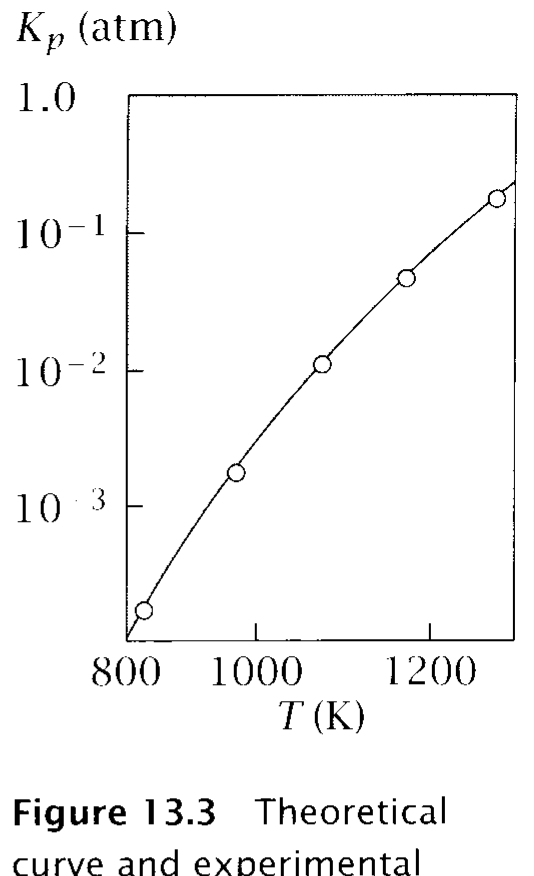
\includegraphics[width=0.6\textwidth]{figs/iodo.png}
\end{frame}
\begin{frame}{Resposta a Perturbações}
        Qualquer perturbação de um estado de equilíbrio estável deve aumentar a energia livre do sistema. O sistema responderá movendo-se de volta ao estado de equilíbrio.
        
        Para $A \rightleftharpoons B$, se uma flutuação muda $N_B$ por $dN_B$:
        $$ dG = (\mu_B - \mu_A)dN_B $$
        
        
\end{frame}
\begin{frame}{Resposta a Perturbações}
        Qualquer perturbação de um estado de equilíbrio estável deve aumentar a energia livre do sistema. O sistema responderá movendo-se de volta ao estado de equilíbrio.
        Para se mover em direção ao equilíbrio, $dG \le 0$.
        Se $\mu_B > \mu_A$, então $dN_B < 0$ (para $dG < 0$), significando que $N_B$ diminuirá.
        O potencial químico é às vezes chamado de "tendência de escape".
        
\end{frame}
\begin{frame}{Resposta a Perturbações}
        \textbf{Princípio de Le Chatelier:} Um sistema em equilíbrio, quando perturbado, ajusta-se de forma a minimizar o efeito da perturbação e retornar ao equilíbrio.
        \begin{figure}
        \centering
        % Conceptual representation of Figure 13.4
        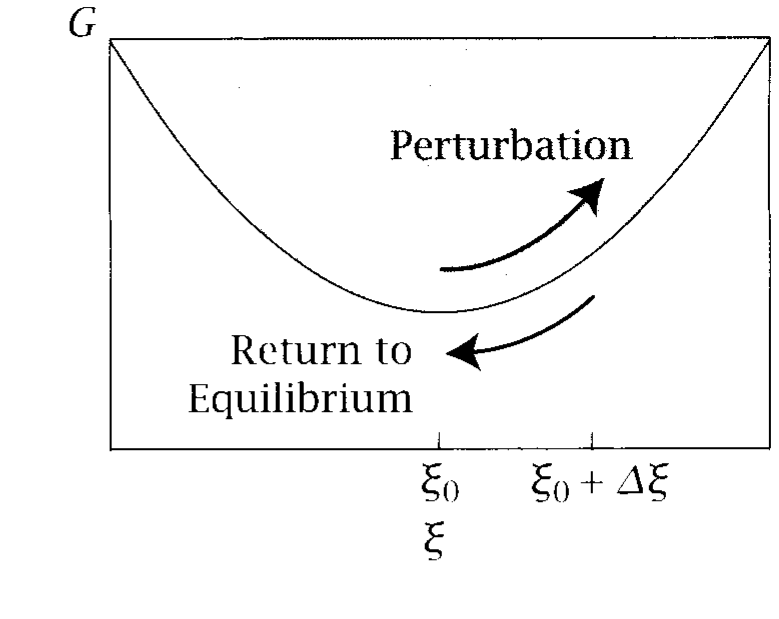
\includegraphics[width=0.6\textwidth]{figs/lechatelier.png}
        \caption{Para a reação $A \rightarrow B$, uma flutuação que aumenta B (aumentando $\xi$) leva o sistema a retornar ao equilíbrio reduzindo a quantidade de B.}
        \end{figure}
\end{frame}

\begin{frame}{Dependência da Temperatura do Equilíbrio: Equação de van 't Hoff}
    Medir $K(T)$ em diferentes temperaturas permite determinar $\Delta h^{\circ}$ e $\Delta s^{\circ}$ da reação.
    No equilíbrio, $\mu_A = \mu_B$. Usando $\mu = \mu^{\circ} + kT \ln p$:
    $$ \mu_A^{\circ} + kT \ln p_A = \mu_B^{\circ} + kT \ln p_B $$
    $$ \ln K_p = \ln\left(\frac{p_B}{p_A}\right) = -\frac{(\mu_B^{\circ} - \mu_A^{\circ})}{kT} = -\frac{\Delta\mu^{\circ}}{kT} $$
     
\end{frame}

\begin{frame}{Dependência da Temperatura do Equilíbrio: Equação de van 't Hoff}
    Como $\Delta\mu^{\circ} = \Delta h^{\circ} - T\Delta s^{\circ}$:
    $$ \ln K_p = -\frac{\Delta h^{\circ}}{kT} + \frac{\Delta s^{\circ}}{k} $$
     
    A dependência com a temperatura é (assumindo $\Delta h^{\circ}$ e $\Delta s^{\circ}$ independentes de T):
    $$ \left(\frac{\partial \ln K_p}{\partial T}\right)_p = \frac{\Delta h^{\circ}}{kT^2} $$
     
\end{frame}

\begin{frame}{Dependência da Temperatura do Equilíbrio: Equação de van 't Hoff}
    Forma alternativa (relação de van 't Hoff), usando $d(1/T) = -(1/T^2)dT$:
    $$ \left(\frac{\partial \ln K_p}{\partial (1/T)}\right)_p = -\frac{\Delta h^{\circ}}{k} $$
    
    Um gráfico de $\ln K_p$ versus $1/T$ (gráfico de van 't Hoff) tem inclinação $-\Delta h^{\circ}/k$.
\end{frame}

\begin{frame}{Gráfico de van 't Hoff e Integração}
    \begin{figure}
    \centering
    % Conceptual representation of Figure 13.5
    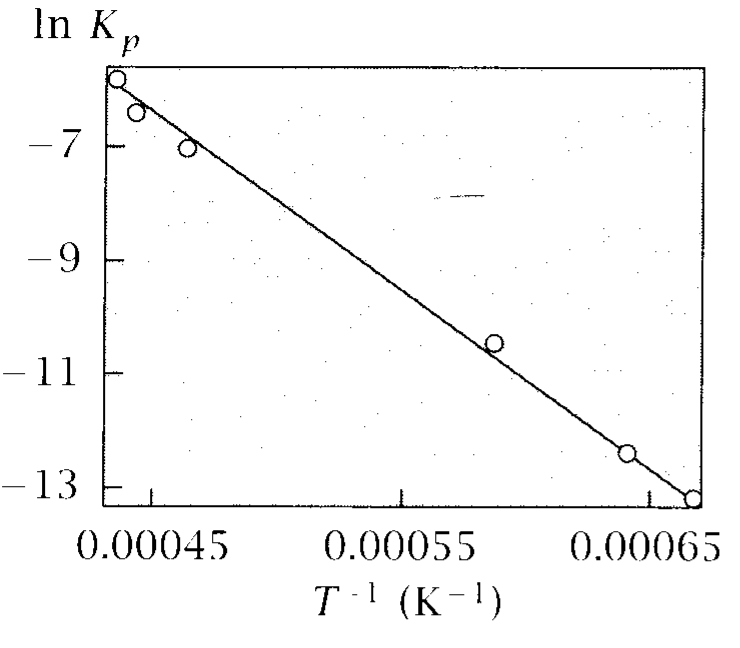
\includegraphics[width=0.7\textwidth]{figs/hoff.png}
    \caption{Gráfico de van 't Hoff para a dissociação da água. A linearidade sugere que $\Delta h^{\circ}$ é aproximadamente constante na faixa de temperatura.}
    \end{figure}
    
\end{frame}

\begin{frame}{Gráfico de van 't Hoff e Integração}
    Se $\Delta h^{\circ}$ é independente da temperatura, a integração da equação de van 't Hoff resulta em:
    $$ \ln\left(\frac{K_p(T_2)}{K_p(T_1)}\right) = -\frac{\Delta h^{\circ}}{k}\left(\frac{1}{T_2} - \frac{1}{T_1}\right) $$
     
\end{frame}

\begin{frame}{Gráfico de van 't Hoff e Integração}
    Obtendo $\Delta h^{\circ}$ de um gráfico de van 't Hoff 
        Para a dissociação da água, usando dois pontos de Fig. 13.5:
        $(1/T_1, \ln K_{p1}) = (6.66 \times 10^{-4} K^{-1}, -13.147)$ ($T_1=1500K$)
        $(1/T_2, \ln K_{p2}) = (4.43 \times 10^{-4} K^{-1}, -6.4)$ ($T_2=2257K$)
        $$ \Delta h^{\circ} = \frac{-R[\ln K_p(T_2) - \ln K_p(T_1)]}{(1/T_2) - (1/T_1)} = 249 \text{ kJ mol}^{-1} $$
        
        Também se pode obter $\Delta\mu^{\circ}$ e $\Delta s^{\circ}$.
\end{frame}

\begin{frame}{Equação de Gibbs-Helmholtz}
    Para uma dependência geral da energia livre $G(T)$ com a temperatura:
    Sabemos que $H = G + TS$ e $S = -(\partial G/\partial T)_p$.
    Substituindo S:
    $$ H = G - T\left(\frac{\partial G}{\partial T}\right)_p $$
     
\end{frame}

\begin{frame}{Equação de Gibbs-Helmholtz}
    Considerando a derivada de $G/T$ em relação a T:
    $$ \left(\frac{\partial (G/T)}{\partial T}\right)_p = \frac{1}{T}\left(\frac{\partial G}{\partial T}\right)_p - \frac{G}{T^2} = -\frac{1}{T^2}\left(G - T\left(\frac{\partial G}{\partial T}\right)_p\right) $$
     
    Substituindo a expressão de H, obtemos a equação de Gibbs-Helmholtz:
    $$ \left(\frac{\partial (G/T)}{\partial T}\right)_p = -\frac{H(T)}{T^2} $$
    
\end{frame}

\begin{frame}{Equação de Gibbs-Helmholtz}
    Similarmente, para a energia livre de Helmholtz F:
    $$ \left(\frac{\partial (F/T)}{\partial T}\right)_V = -\frac{U(T)}{T^2} $$
    
    Estas equações são válidas mesmo quando $\Delta h^{\circ}$ depende da temperatura.
\end{frame}

\begin{frame}{Dependência da Constante de Equilíbrio com a Pressão}
    A dependência de $K(p)$ com a pressão reflete uma mudança de volume.
    $$ \frac{\partial \ln K(p)}{\partial p} = \frac{\partial}{\partial p}\left[-\frac{(\mu_B^{\circ} - \mu_A^{\circ})}{kT}\right] = -\frac{1}{kT}\left(\frac{\partial \Delta\mu^{\circ}}{\partial p}\right)_T $$
     
\end{frame}

\begin{frame}{Dependência da Constante de Equilíbrio com a Pressão}
    Da equação de Gibbs-Duhem ($N_A d\mu_A = Vdp - SdT$), para uma única espécie A: $d\mu_A = v_A dp - s_A dT$, onde $v_A$ é o volume molar.
    Então, $d(\mu_B^{\circ} - \mu_A^{\circ}) = (v_B - v_A)dp - (s_B - s_A)dT$.
    $$ \left(\frac{\partial(\mu_B^{\circ} - \mu_A^{\circ})}{\partial p}\right)_T = v_B - v_A = \Delta v $$
     
\end{frame}

\begin{frame}{Dependência da Constante de Equilíbrio com a Pressão}
    Substituindo na derivada de $\ln K$:
    $$ \left(\frac{\partial \ln K}{\partial p}\right)_T = -\frac{\Delta v}{kT} $$
    
    Se B é o estado com menor volume ($\Delta v < 0$), aumentar a pressão deslocará o equilíbrio de A para B.
\end{frame}

\begin{frame}{Halotano: Água $\rightleftharpoons$ Membrana Lipídica (Exemplo 13.6 )}
    Halotano: Água $\rightleftharpoons$ Membrana Lipídica 
        O anestésico halotano particiona entre água (estado A) e membranas de bicamada lipídica (estado B).
        A Figura 13.6 mostra como o equilíbrio de partição $K$ (coeficiente de partição da água para a bicamada ) depende da pressão.
\end{frame}

\begin{frame}{Halotano: Água $\rightleftharpoons$ Membrana Lipídica (Exemplo 13.6 )}
        \begin{figure}
        \centering
        % Conceptual representation of Figure 13.6
        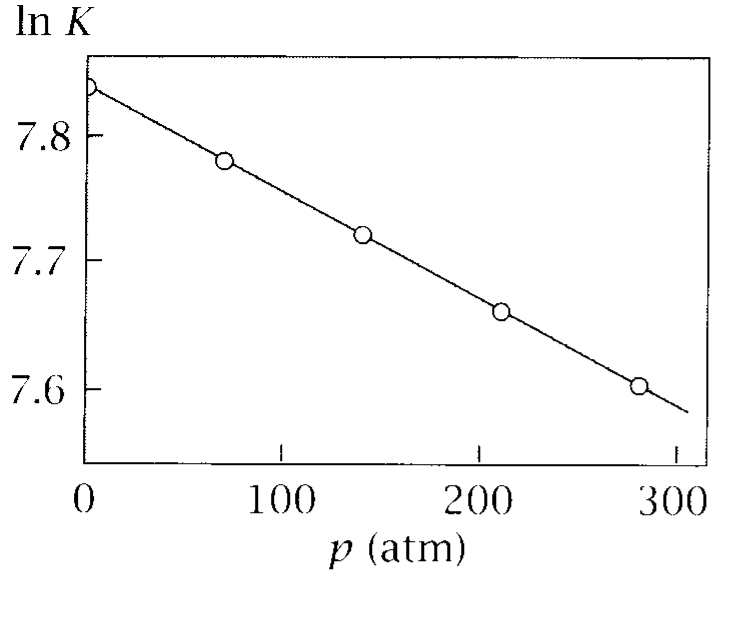
\includegraphics[width=0.6\textwidth]{figs/pressure_K.png}
        \caption{Aplicar pressão desloca moléculas de anestésico para a água a partir de membranas de bicamada lipídica.}
        \end{figure}
        
\end{frame}

\begin{frame}{Halotano: Água $\rightleftharpoons$ Membrana Lipídica (Exemplo 13.6 )}
        Usando pontos $(p_1, \ln K_1) = (0 \text{ atm}, 7.84)$ e $(p_2, \ln K_2) = (280 \text{ atm}, 7.60)$ a $T=300K$:
        $$ \Delta v = v_{\text{bicamada}} - v_{\text{água}} = -RT \frac{(\ln K_2 - \ln K_1)}{p_2 - p_1} $$
        
        $$ \Delta v = \frac{-(8.205 \times 10^{-5} m^3 atm K^{-1} mol^{-1})(300K)(7.60 - 7.84)}{280 atm - 0 atm} $$
        $$ \Delta v \approx 2.1 \times 10^{-5} m^3 mol^{-1} = 21 cm^3 mol^{-1} $$
        
\end{frame}

\begin{frame}{Halotano: Água $\rightleftharpoons$ Membrana Lipídica (Exemplo 13.6 )}
        Isso corresponde a uma variação de volume de $35 \AA^3$ por molécula. O anestésico ocupa mais volume na fase de membrana. A pressão força as moléculas de anestésico para a água, onde ocupam volumes menores.
\end{frame}

\begin{frame}{Resumo}
    \begin{itemize}
        \item Uma conquista notável da mecânica estatística é a previsão precisa dos equilíbrios de reações químicas em fase gasosa a partir de estruturas atômicas.
        \item A partir de massas atômicas, momentos de inércia, comprimentos de ligação e forças de ligação, pode-se calcular funções de partição.
        \item Com as funções de partição, é possível calcular constantes de equilíbrio e sua dependência da temperatura e pressão.
    \end{itemize}
\end{frame}

% Placeholder images (create these files or replace with actual paths)
% placeholder_energylevels.png
% placeholder_lechatelier.png
% placeholder_vanthoff.png
% placeholder_pressure_K.png
% You would typically create these image files (e.g., as PNG or PDF).
% For this example, let's assume they are simple conceptual drawings.
% If you have the actual figures from the PDF as image files, you can use them.

\end{document}
